Baseando-se nos passos anteriores, onde atividades foram excluídas e incluídas, simplificando o sequenciamento do processo bem como facilitando seu entendimento, o seguinte modelo TO-BE foi desenvolvido por completo na sua primeira versão:
\begin{figure}[H]
	\centering
	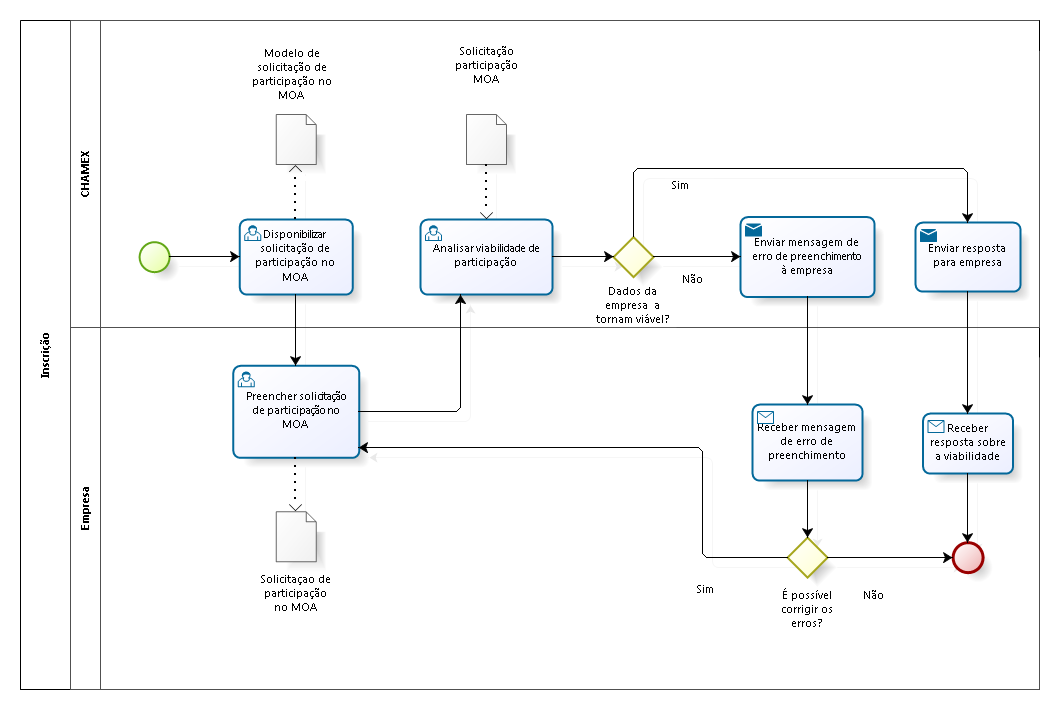
\includegraphics[scale=0.55]{to-be_1}
	\label{fig:tobeversaoum}
	\caption[Primeira Versão do Modelo TO-BE]{Primeira Versão do Modelo TO-BE.}
\end{figure}
É possível verificar que a atividade onde a empresa avalia se deseja ou não corrigir os erros de preenchimento ainda não existia nessa versão. Em seguida, em um processo iterativo onde buscou-se melhorar ainda mais o processo, o modelo continuou passando por modificações até chegar na sua quinta versão, esta sim apresentando evoluções consideráveis como a atividade e o gateway que definem o rumo que a empresa irá tomar caso sua solicitação tenha sido rejeitada por erro de preenchimento. Além disso foi criada a atividade atribuir solicitação para avaliação antes da atividade que define a análise realizada, dando mais clareza ao processo no que diz respeito a distribuição de atividades em diferentes papéis.
\begin{figure}[H]
	\centering
	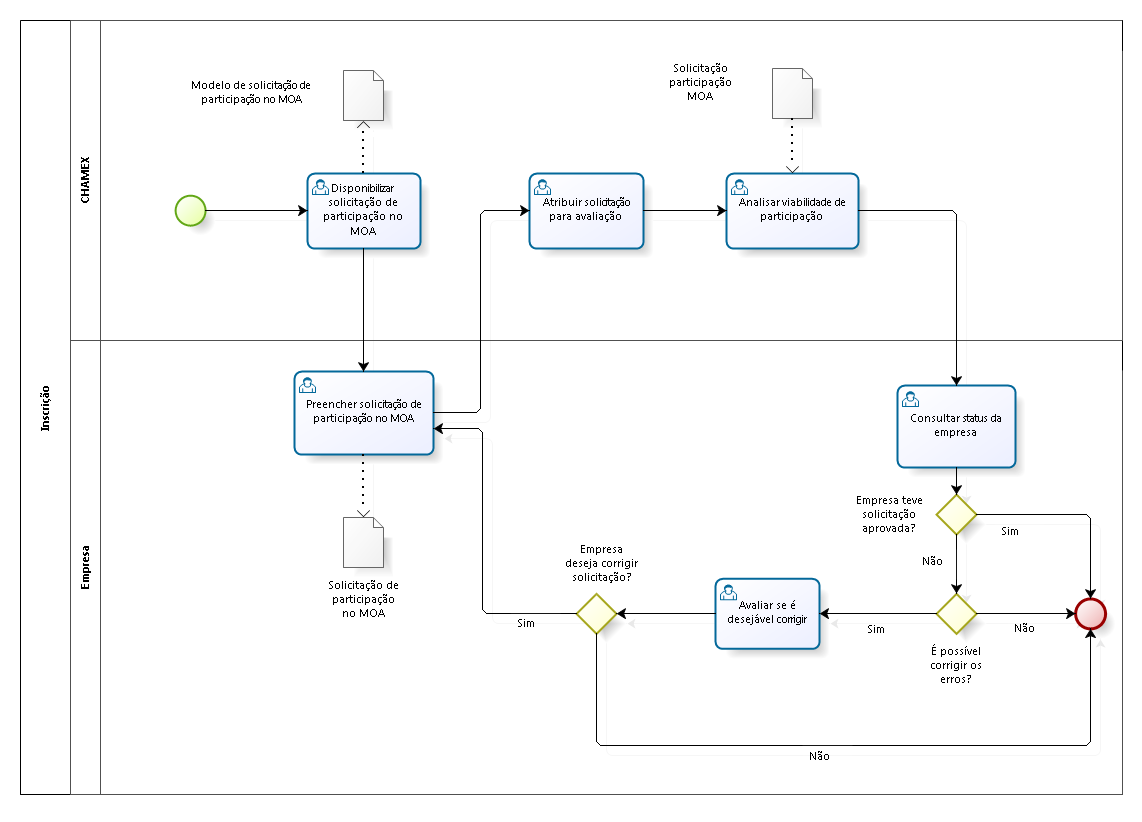
\includegraphics[scale=0.5]{to-be_5}
	\label{fig:tobeversaofinal}
	\caption[Quinta Versão (Final) do Modelo TO-BE]{Quinta Versão (Final) do Modelo TO-BE.}
\end{figure}
As três atividades incluídas são descritas da seguinte maneira:
\begin{itemize}
	\item{\textbf{Consultar \emph{Status} da Empresa}: Empresa realiza consulta no site do MOA a respeito do status da sua solicitação (aprovada ou rejeitada);}
	\item{\textbf{Avaliar se é Desejável Corrigir}: Empresa avalia com base nos resultados emitidos pelo \emph{check-list} da solicitação realizado pelo analisador do MOA se é desejável corrigir os erros com o objetivo de novamente ter sua solicitação analisado ou se é preferível não corrigir os erros e abandonar o processo de inscrição;}
	\item{\textbf{Atribuir a Solicitaçao para Avaliação}: Gerente do MOA atribui a solictação para ser validada por um analista a ser escolhido por ele.}
\end{itemize}